%\documentclass[preprint,3p,times,twocolumn]{elsarticleUS}
\documentclass[review,3p,times]{elsarticleUS}
%\documentclass{article}

\usepackage{amssymb}
\usepackage{amsmath}
\usepackage{graphicx}
\usepackage{bm}
\usepackage{yhmath}
\usepackage{subfigure}
\usepackage{multirow}
\usepackage{color}
\usepackage{xcolor}
\usepackage{subdepth}



\biboptions{comma,sort&compress}

\journal{Proceedings of the Combustion Institute}

\makeatletter
\def\@author#1{\g@addto@macro\elsauthors{\normalsize%
    \def\baselinestretch{1}%
    \upshape\authorsep#1\unskip\textsuperscript{%
      \ifx\@fnmark\@empty\else\unskip\sep\@fnmark\let\sep=,\fi
      \ifx\@corref\@empty\else\unskip\sep\@corref\let\sep=,\fi
      }%
    \def\authorsep{\unskip,\space}%
    \global\let\@fnmark\@empty
    \global\let\@corref\@empty  %% Added
    \global\let\sep\@empty}%
    \@eadauthor={#1}
}
\makeatother

\begin{document}

\begin{frontmatter}

\title{Sooting Limits of Nonpremixed $n$-Heptane, $n$-Butanol and Methyl Butanoate}

\author{Sili~Deng\corref{cor}}
\cortext[cor]{Corresponding Author: silideng@princeton.edu}
\author{Jeremy A.~Koch}
\author{Michael E.~Mueller}
\author{Chung K.~Law}

\address{Department of Mechanical and Aerospace Engineering, Princeton University, Princeton, NJ 08544, USA}

\end{frontmatter}


\section*{Supplemental Materials}

%\begin{table}
%  \caption{Oxidizer stream composition in molecular fractions.}
%  \label{table:exp_condition_2}
%  \centering
%  \begin{tabular}{cccccc}
%    \hline
%     & $n-C_7H_{16}$ & \multicolumn{2}{c}{$n-C_4H_9OH$} & \multicolumn{2}{c}{$C_5H_{10}O_2$} \\
%    \cline{2-6}
%    $O_2$ & $N_2$ & $N_2$ & $Ar$ & $N_2$ & $Ar$ \\
%    \hline
%    $0.1800$ & $0.8200$ \\
%    $0.1850$ & $0.8150$ \\
%    $0.1875$ & $0.8125$ \\
%    $0.1900$ & $0.8100$ \\
%    $0.1925$ & $0.8075$ \\
%    $0.1950$ & $0.8050$ & $0.7718$ & $0.0332$ \\
%    $0.1975$ &          & $0.7679$ & $0.0346$ \\
%    $0.2000$ & $0.8000$ & $0.7640$ & $0.0360$ \\
%    $0.2025$ &          & $0.7600$ & $0.0374$ \\
%    $0.2050$ &          & $0.7560$ & $0.0390$ & $0.7119$ & $0.0831$ \\
%    $0.2075$ &          & $0.7521$ & $0.0404$ \\
%    $0.2100$ &          &          &          & $0.7017$ & $0.0883$ \\
%    $0.2150$ &          &          &          & $0.6915$ & $0.0935$ \\
%    $0.2200$ &          &          &          & $0.6811$ & $0.0989$ \\
%    $0.2250$ &          &          &          & $0.6707$ & $0.1043$ \\
%    \hline
%  \end{tabular}
%\end{table}


\begin{table*}[h]
  \caption{X$_{O_2}$ in the oxidizer at experimental conditions.}
  \label{table:exp_condition}
  \centering
  \resizebox{1.0\textwidth}{!}{
  \begin{tabular}{ll*{15}{c}}
    \hline
     & \multicolumn{16}{c}{$O_2$} \\
    \cline{3-17}
     &  & $0.1800$ & $0.1850$ & $0.1875$ & $0.1900$ & $0.1925$ & $0.1950$ & $0.1975$ & $0.2000$ & $0.2025$ & $0.2050$ & $0.2075$ & $0.2100$ & $0.2150$ & $0.2200$ & $0.2250$ \\
    \hline
    $n-C_7H_{16}$ & $N_2$ &  $0.8200$ & $0.8150$ & $0.8125$ & $0.8100$ & $0.8075$ & $0.8050$ &  & $0.8000$ \\
    %%    \hline
    %%    \multirow{2}{*}{$n-C_4H_9OH$} & $N_2$ &  &   &  &  &  & $0.7718$ & $0.7679$ & $0.7640$ & $0.7600$ & $0.7560$ & $0.7521$ \\
    $n-C_4H_9OH$ & $N_2$ &  &   &  &  &  & $0.7718$ & $0.7679$ & $0.7640$ & $0.7600$ & $0.7560$ & $0.7521$ \\
                 & $Ar$ &  &  &  &  &  & $0.0332$ & $0.0346$ & $0.0360$ & $0.0375$ & $0.0390$ & $0.0404$ \\
    %%    \hline
    %%    \multirow{2}{*}{$C_5H_{10}O_2$} & $N_2$ & & & & & & & & & & $0.7119$ & & $0.7017$ & $0.6915$ & $0.6811$ & $0.6707$ \\
    $C_5H_{10}O_2$ & $N_2$ & & & & & & & & & & $0.7119$ & & $0.7017$ & $0.6915$ & $0.6811$ & $0.6707$ \\
                 & $Ar$ &  &  &  &  &  & & & & & $0.0831$ & & $0.0883$ & $0.0935$ & $0.0989$ & $0.1043$ \\ 
    \hline
  \end{tabular}
}
\end{table*}


\begin{figure*}[p]
  \centering
  \scriptsize
%  \vspace{-0.1in}
  % GNUPLOT: LaTeX picture with Postscript
\begingroup
  \makeatletter
  \providecommand\color[2][]{%
    \GenericError{(gnuplot) \space\space\space\@spaces}{%
      Package color not loaded in conjunction with
      terminal option `colourtext'%
    }{See the gnuplot documentation for explanation.%
    }{Either use 'blacktext' in gnuplot or load the package
      color.sty in LaTeX.}%
    \renewcommand\color[2][]{}%
  }%
  \providecommand\includegraphics[2][]{%
    \GenericError{(gnuplot) \space\space\space\@spaces}{%
      Package graphicx or graphics not loaded%
    }{See the gnuplot documentation for explanation.%
    }{The gnuplot epslatex terminal needs graphicx.sty or graphics.sty.}%
    \renewcommand\includegraphics[2][]{}%
  }%
  \providecommand\rotatebox[2]{#2}%
  \@ifundefined{ifGPcolor}{%
    \newif\ifGPcolor
    \GPcolortrue
  }{}%
  \@ifundefined{ifGPblacktext}{%
    \newif\ifGPblacktext
    \GPblacktexttrue
  }{}%
  % define a \g@addto@macro without @ in the name:
  \let\gplgaddtomacro\g@addto@macro
  % define empty templates for all commands taking text:
  \gdef\gplbacktext{}%
  \gdef\gplfronttext{}%
  \makeatother
  \ifGPblacktext
    % no textcolor at all
    \def\colorrgb#1{}%
    \def\colorgray#1{}%
  \else
    % gray or color?
    \ifGPcolor
      \def\colorrgb#1{\color[rgb]{#1}}%
      \def\colorgray#1{\color[gray]{#1}}%
      \expandafter\def\csname LTw\endcsname{\color{white}}%
      \expandafter\def\csname LTb\endcsname{\color{black}}%
      \expandafter\def\csname LTa\endcsname{\color{black}}%
      \expandafter\def\csname LT0\endcsname{\color[rgb]{1,0,0}}%
      \expandafter\def\csname LT1\endcsname{\color[rgb]{0,1,0}}%
      \expandafter\def\csname LT2\endcsname{\color[rgb]{0,0,1}}%
      \expandafter\def\csname LT3\endcsname{\color[rgb]{1,0,1}}%
      \expandafter\def\csname LT4\endcsname{\color[rgb]{0,1,1}}%
      \expandafter\def\csname LT5\endcsname{\color[rgb]{1,1,0}}%
      \expandafter\def\csname LT6\endcsname{\color[rgb]{0,0,0}}%
      \expandafter\def\csname LT7\endcsname{\color[rgb]{1,0.3,0}}%
      \expandafter\def\csname LT8\endcsname{\color[rgb]{0.5,0.5,0.5}}%
    \else
      % gray
      \def\colorrgb#1{\color{black}}%
      \def\colorgray#1{\color[gray]{#1}}%
      \expandafter\def\csname LTw\endcsname{\color{white}}%
      \expandafter\def\csname LTb\endcsname{\color{black}}%
      \expandafter\def\csname LTa\endcsname{\color{black}}%
      \expandafter\def\csname LT0\endcsname{\color{black}}%
      \expandafter\def\csname LT1\endcsname{\color{black}}%
      \expandafter\def\csname LT2\endcsname{\color{black}}%
      \expandafter\def\csname LT3\endcsname{\color{black}}%
      \expandafter\def\csname LT4\endcsname{\color{black}}%
      \expandafter\def\csname LT5\endcsname{\color{black}}%
      \expandafter\def\csname LT6\endcsname{\color{black}}%
      \expandafter\def\csname LT7\endcsname{\color{black}}%
      \expandafter\def\csname LT8\endcsname{\color{black}}%
    \fi
  \fi
  \setlength{\unitlength}{0.0500bp}%
  \begin{picture}(7200.00,5040.00)%
    \gplgaddtomacro\gplbacktext{%
      \csname LTb\endcsname%
      \put(814,704){\makebox(0,0)[r]{\strut{} 0}}%
      \put(814,1074){\makebox(0,0)[r]{\strut{} 5}}%
      \put(814,1444){\makebox(0,0)[r]{\strut{} 10}}%
      \put(814,1814){\makebox(0,0)[r]{\strut{} 15}}%
      \put(814,2184){\makebox(0,0)[r]{\strut{} 20}}%
      \put(814,2554){\makebox(0,0)[r]{\strut{} 25}}%
      \put(814,2925){\makebox(0,0)[r]{\strut{} 30}}%
      \put(814,3295){\makebox(0,0)[r]{\strut{} 35}}%
      \put(814,3665){\makebox(0,0)[r]{\strut{} 40}}%
      \put(814,4035){\makebox(0,0)[r]{\strut{} 45}}%
      \put(814,4405){\makebox(0,0)[r]{\strut{} 50}}%
      \put(814,4775){\makebox(0,0)[r]{\strut{} 55}}%
      \put(946,484){\makebox(0,0){\strut{} 0.4}}%
      \put(1678,484){\makebox(0,0){\strut{} 0.6}}%
      \put(2410,484){\makebox(0,0){\strut{} 0.8}}%
      \put(3142,484){\makebox(0,0){\strut{} 1}}%
      \put(3874,484){\makebox(0,0){\strut{} 1.2}}%
      \put(4607,484){\makebox(0,0){\strut{} 1.4}}%
      \put(5339,484){\makebox(0,0){\strut{} 1.6}}%
      \put(6071,484){\makebox(0,0){\strut{} 1.8}}%
      \put(6803,484){\makebox(0,0){\strut{} 2}}%
      \put(176,2739){\rotatebox{-270}{\makebox(0,0){\strut{}Laminar Flame Speeds (cm/s)}}}%
      \put(3874,154){\makebox(0,0){\strut{}$\phi$}}%
    }%
    \gplgaddtomacro\gplfronttext{%
      \csname LTb\endcsname%
      \put(5816,4602){\makebox(0,0)[r]{\strut{}Liu}}%
      \csname LTb\endcsname%
      \put(5816,4382){\makebox(0,0)[r]{\strut{}Present work}}%
      \csname LTb\endcsname%
      \put(5816,4162){\makebox(0,0)[r]{\strut{}Liu}}%
    }%
    \gplbacktext
    \put(0,0){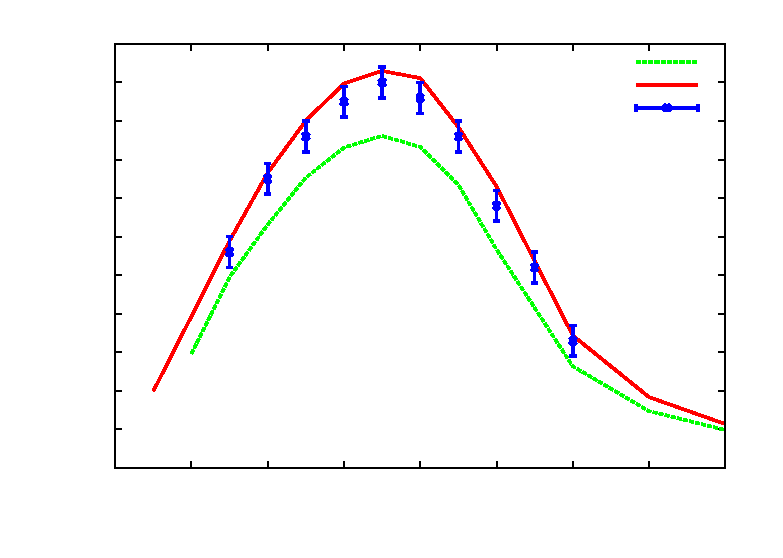
\includegraphics{BV_NB}}%
    \gplfronttext
  \end{picture}%
\endgroup

  \normalsize
%  \vspace{-0.2in}
  \caption{Mechanism validation on $n$-butanol laminar flame speeds, against the experimental (symbols) and computational (dotted lines) results in Ref.[1]. $P=1 atm$ and $T=353 K$.}
  \label{fig:BV_NB}
\end{figure*}

\begin{figure*}[p]
  \centering
  \scriptsize
%  \vspace{-0.1in}
  % GNUPLOT: LaTeX picture with Postscript
\begingroup
  \makeatletter
  \providecommand\color[2][]{%
    \GenericError{(gnuplot) \space\space\space\@spaces}{%
      Package color not loaded in conjunction with
      terminal option `colourtext'%
    }{See the gnuplot documentation for explanation.%
    }{Either use 'blacktext' in gnuplot or load the package
      color.sty in LaTeX.}%
    \renewcommand\color[2][]{}%
  }%
  \providecommand\includegraphics[2][]{%
    \GenericError{(gnuplot) \space\space\space\@spaces}{%
      Package graphicx or graphics not loaded%
    }{See the gnuplot documentation for explanation.%
    }{The gnuplot epslatex terminal needs graphicx.sty or graphics.sty.}%
    \renewcommand\includegraphics[2][]{}%
  }%
  \providecommand\rotatebox[2]{#2}%
  \@ifundefined{ifGPcolor}{%
    \newif\ifGPcolor
    \GPcolortrue
  }{}%
  \@ifundefined{ifGPblacktext}{%
    \newif\ifGPblacktext
    \GPblacktexttrue
  }{}%
  % define a \g@addto@macro without @ in the name:
  \let\gplgaddtomacro\g@addto@macro
  % define empty templates for all commands taking text:
  \gdef\gplbacktext{}%
  \gdef\gplfronttext{}%
  \makeatother
  \ifGPblacktext
    % no textcolor at all
    \def\colorrgb#1{}%
    \def\colorgray#1{}%
  \else
    % gray or color?
    \ifGPcolor
      \def\colorrgb#1{\color[rgb]{#1}}%
      \def\colorgray#1{\color[gray]{#1}}%
      \expandafter\def\csname LTw\endcsname{\color{white}}%
      \expandafter\def\csname LTb\endcsname{\color{black}}%
      \expandafter\def\csname LTa\endcsname{\color{black}}%
      \expandafter\def\csname LT0\endcsname{\color[rgb]{1,0,0}}%
      \expandafter\def\csname LT1\endcsname{\color[rgb]{0,1,0}}%
      \expandafter\def\csname LT2\endcsname{\color[rgb]{0,0,1}}%
      \expandafter\def\csname LT3\endcsname{\color[rgb]{1,0,1}}%
      \expandafter\def\csname LT4\endcsname{\color[rgb]{0,1,1}}%
      \expandafter\def\csname LT5\endcsname{\color[rgb]{1,1,0}}%
      \expandafter\def\csname LT6\endcsname{\color[rgb]{0,0,0}}%
      \expandafter\def\csname LT7\endcsname{\color[rgb]{1,0.3,0}}%
      \expandafter\def\csname LT8\endcsname{\color[rgb]{0.5,0.5,0.5}}%
    \else
      % gray
      \def\colorrgb#1{\color{black}}%
      \def\colorgray#1{\color[gray]{#1}}%
      \expandafter\def\csname LTw\endcsname{\color{white}}%
      \expandafter\def\csname LTb\endcsname{\color{black}}%
      \expandafter\def\csname LTa\endcsname{\color{black}}%
      \expandafter\def\csname LT0\endcsname{\color{black}}%
      \expandafter\def\csname LT1\endcsname{\color{black}}%
      \expandafter\def\csname LT2\endcsname{\color{black}}%
      \expandafter\def\csname LT3\endcsname{\color{black}}%
      \expandafter\def\csname LT4\endcsname{\color{black}}%
      \expandafter\def\csname LT5\endcsname{\color{black}}%
      \expandafter\def\csname LT6\endcsname{\color{black}}%
      \expandafter\def\csname LT7\endcsname{\color{black}}%
      \expandafter\def\csname LT8\endcsname{\color{black}}%
    \fi
  \fi
  \setlength{\unitlength}{0.0500bp}%
  \begin{picture}(7200.00,5040.00)%
    \gplgaddtomacro\gplbacktext{%
      \csname LTb\endcsname%
      \put(814,704){\makebox(0,0)[r]{\strut{} 5}}%
      \put(814,1111){\makebox(0,0)[r]{\strut{} 10}}%
      \put(814,1518){\makebox(0,0)[r]{\strut{} 15}}%
      \put(814,1925){\makebox(0,0)[r]{\strut{} 20}}%
      \put(814,2332){\makebox(0,0)[r]{\strut{} 25}}%
      \put(814,2740){\makebox(0,0)[r]{\strut{} 30}}%
      \put(814,3147){\makebox(0,0)[r]{\strut{} 35}}%
      \put(814,3554){\makebox(0,0)[r]{\strut{} 40}}%
      \put(814,3961){\makebox(0,0)[r]{\strut{} 45}}%
      \put(814,4368){\makebox(0,0)[r]{\strut{} 50}}%
      \put(814,4775){\makebox(0,0)[r]{\strut{} 55}}%
      \put(946,484){\makebox(0,0){\strut{} 0.4}}%
      \put(1678,484){\makebox(0,0){\strut{} 0.6}}%
      \put(2410,484){\makebox(0,0){\strut{} 0.8}}%
      \put(3142,484){\makebox(0,0){\strut{} 1}}%
      \put(3874,484){\makebox(0,0){\strut{} 1.2}}%
      \put(4607,484){\makebox(0,0){\strut{} 1.4}}%
      \put(5339,484){\makebox(0,0){\strut{} 1.6}}%
      \put(6071,484){\makebox(0,0){\strut{} 1.8}}%
      \put(6803,484){\makebox(0,0){\strut{} 2}}%
      \put(176,2739){\rotatebox{-270}{\makebox(0,0){\strut{}Laminar Flame Speeds (cm/s)}}}%
      \put(3874,154){\makebox(0,0){\strut{}$\phi$}}%
    }%
    \gplgaddtomacro\gplfronttext{%
      \csname LTb\endcsname%
      \put(5816,4602){\makebox(0,0)[r]{\strut{}Liu}}%
      \csname LTb\endcsname%
      \put(5816,4382){\makebox(0,0)[r]{\strut{}Present work}}%
      \csname LTb\endcsname%
      \put(5816,4162){\makebox(0,0)[r]{\strut{}Liu}}%
    }%
    \gplbacktext
    \put(0,0){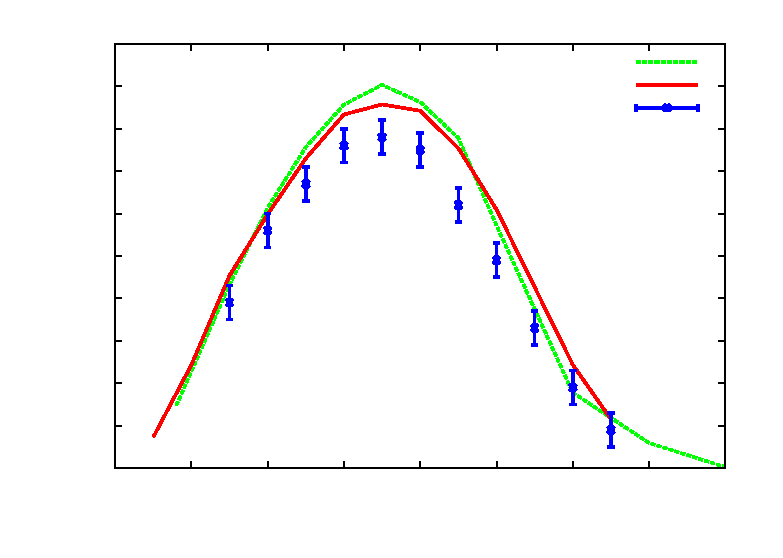
\includegraphics{BV_MB}}%
    \gplfronttext
  \end{picture}%
\endgroup

  \normalsize
%  \vspace{-0.2in}
  \caption{Mechanism validation on methyl butanoate laminar flame speeds, against the experimental (symbols) and computational (dotted lines) results in Ref.[1]. $P=1 atm$ and $T=353 K$.}
  \label{fig:BV_MB}
\end{figure*}

\end{document}

